% June 2015 (TOC contents linked in blue in pdf file)
%This template was prepared by Dorothea F. Brosius of the
%Institute for Electronics and Applied Physics, University of Maryland, College Park, MD
%The template was last updated in June 2015
%Thesis Main Page used with thesis.sty based on the
%University of Maryland Electronic Thesis and Dissertation (ETD) Style Guide (2014)

%The YourInformation file was created by Freja Nordsiek, 2014.
%Code for linking the TOC titles to the text in the pdf file was created by Freja Nordsiek, 2014.

%Code clean-up and addition of glossaries by Patrick Stanley, 2017.
%Assumed printing to pdf and extra sections not needed (such as preface and forward)

\documentclass[12pt]{thesis}

%some packages may not be needed depending on your use
\usepackage{titlesec}
   \titleformat{\chapter}
      {\normalfont\large}{Chapter \thechapter:}{1em}{}
\usepackage{lipsum} %Remove before final draft, used to generate filler text
\usepackage{graphicx}
  \graphicspath{ {Images/} } %defining where images go here so I don't have to every time
\usepackage{cite}
\usepackage{lscape}
\usepackage{indentfirst}
\usepackage{latexsym}
\usepackage{multirow}
\usepackage{tabls}
\usepackage{wrapfig}%for wrapping text around figures in the document; don't need figure wrapping in this document
\usepackage{longtable}
\usepackage{supertabular}%for large tables that do not fit on a single page; also probably won't need this
%\usepackage{subeqn} %removed to fix error with glossaries package
\usepackage{subfigure}%allows creation of subfigures (i.e.  Fig #a, Fig. #b...)
\usepackage{microtype}%readablity enhancements
\usepackage[bookmarks, colorlinks=true, plainpages=false, pdfpagelabels, citecolor=blue, urlcolor=blue, filecolor=blue, linkcolor=blue]{hyperref} %creates hyperlinks to various sections in pdf
\usepackage[toc, nonumberlist]{glossaries} %needs to be after hyperref

\newcommand{\tbsp}{\rule{0pt}{18pt}} %used to get a vertical distance after \hline
\renewcommand{\baselinestretch}{2}
\setlength{\textwidth}{5.9in}
\setlength{\textheight}{9in}
\setlength{\topmargin}{-.50in}
\setlength{\oddsidemargin}{.55in}
\setlength{\parindent}{.4in}
\pagestyle{empty}


\setacronymstyle{long-short} %first use of acronym gives full name
\glsdisablehyper %turns off hyperlinking
\loadglsentries{definitions} %defines file with all entries
\renewcommand{\glossarysection}[2][]{} %Hides glossary title so it can be named manually
\makeglossaries


\begin{document}
\hypersetup{pageanchor=false} %Fixes hyperref error with unnumbered title pages
% !TEX root = ../mainthesis.tex

%Abstract Page

\hbox{\ }

\renewcommand{\baselinestretch}{1}
\small \normalsize

\begin{center}
\large{{ABSTRACT}}

\vspace{3em}

\end{center}
\hspace{-.15in}
\begin{tabular}{ll}
Title of dissertation:    & {\large  EVALUATION OF STRENGTH AND  }\\
&				      {\large  RELIABILITY OF SOLID-OXIDE FUEL } \\
&				      {\large  CELLS AT OPERATING CONDITIONS} \\
\ \\
&                          {\large  Patrick Stanley, Doctor of Philosophy, 2018} \\
\ \\
Dissertation directed by: & {\large  Professor Eric D. Wachsman} \\
&  				{\large	 Materials Science and Engineering } \\
\end{tabular}

\vspace{3em}

\renewcommand{\baselinestretch}{2}
\large \normalsize

\lipsum[1-4] %Replace with actual text
 %(must be first, required, non-numbered)
% !TEX root = ../mainthesis.tex

%Titlepage

\thispagestyle{empty}
\hbox{\ }
\vspace{1in}
\renewcommand{\baselinestretch}{1}
\small\normalsize
\begin{center}

\large{{EVALUATION OF STRENGTH AND RELIABILITY OF SOLID-OXIDE FUEL CELLS AT OPERATING CONDITIONS}}\\
\ \\
\ \\
\large{by} \\
\ \\
\large{Patrick Owen Stanley}%Your full name as it appears in University records.
\ \\
\ \\
\ \\
\ \\
\normalsize
Dissertation submitted to the Faculty of the Graduate School of the \\
University of Maryland, College Park in partial fulfillment \\
of the requirements for the degree of \\
Doctor of Philosophy \\
2018
\end{center}

\vspace{7.5em}

\noindent Advisory Committee: \\
Professor Eric D. Wachsman: \textit{Advisor, Chair} \\
Professor Abhijit Dasgupta: \textit{Dean's Representative} \\
Professor Isabel K. Lloyd \\
Professor Lourdes Salamanca-Riba \\
Professor Sreeramamurthy Ankem
 %(must follow Abstract, required, non-numbered)
% !TEX root = ../mainthesis.tex

%Copyright

\thispagestyle{empty}
\hbox{\ }

\vfill
\renewcommand{\baselinestretch}{1}
\small\normalsize

\vspace{-.65in}

\begin{center}
\large{\copyright \hbox{ }Copyright by\\
Patrick Owen Stanley  %Type your name as it appears in University records
\\
2018}
\end{center}

\vfill
 %(highly recommended, non-numbered)

\hypersetup{pageanchor=true}%Pages from this point start at lower-case Roman number ii)
\pagestyle{plain}
\pagenumbering{roman}
\setcounter{page}{2}

%\addcontentsline{toc}{chapter}{Preface}
%\include{Preface}  %(if present, start at lower-case Roman number ii)
%\addcontentsline{toc}{chapter}{Foreword}
%\include{Foreword} %(if present, lower-case Roman)

\newpage
\phantomsection
\addcontentsline{toc}{chapter}{Dedication}%adds to toc so hyperref links correctly
% !TEX root = mainthesis.tex

%Dedication

\renewcommand{\baselinestretch}{2}
\small\normalsize
\hbox{\ }

\vspace{-.65in}

\begin{center}
\large{Dedication}
\end{center}

\noindent I dedicate this work to my wife who has supported and encouraged me throughout.
 %(if present, lower-case Roman)

\newpage
\phantomsection
\addcontentsline{toc}{chapter}{Acknowledgements}%adds to toc so hyperref links correctly
% !TEX root = mainthesis.tex

%Acknowledgments

\renewcommand{\baselinestretch}{2}
\small\normalsize
\hbox{\ }

\vspace{-.65in}

\begin{center}
\large{Acknowledgments}
\end{center}

\vspace{1ex}

\lipsum[2-4] %replace with actual text
 %(if present, lower-case Roman)

\renewcommand{\baselinestretch}{1}
\small\normalsize

\tableofcontents %(required, lower-case Roman)

\newpage
\listoftables %(if present, lower-case Roman)

\newpage
\listoffigures %(if present, lower-case Roman)

\newpage
\phantomsection
\addcontentsline{toc}{chapter}{List of Abbreviations and Symbols} %Manually put in ToC
\renewcommand{\baselinestretch}{1}
\small\normalsize
%\hbox{\ }
\begin{center}
\large{List of Abbreviations and Symbols} %Manually create centered title
\end{center}

\vspace{3pt}

\printglossary


\newpage
\setlength{\parskip}{0em}
\renewcommand{\baselinestretch}{2}
\small\normalsize

%Pages from this point start at Arabic numeral 1
\setcounter{page}{1}
\pagenumbering{arabic}
% !TEX root = mainthesis.tex

%Chapter 1

%\renewcommand{\thechapter}{1}

\chapter{Introduction}

\section{Solid-Oxide Fuel Cells}

This piece will talk about \glspl{sofc}. This is mostly because I work on \glspl{sofc}. %Example of using glossaries package
For a picture of an \gls{sofc} see Figure \ref{image:sofc}.
\begin{figure}[h]
  \centering
  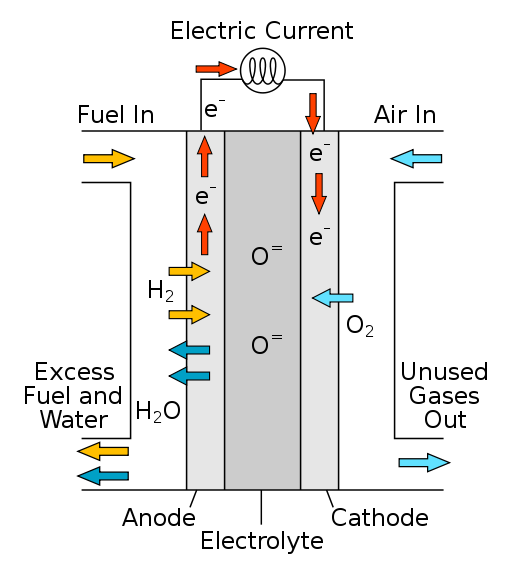
\includegraphics[width=0.5\textwidth]{sofc.png}
  \caption{Diagram showing flow of materials in the operation of a SOFC.\cite{Sakurambo}}
  \label{image:sofc}
\end{figure}

Here is extra text showing how to use various functions.

The response of any dielectric to light becomes nonlinear
for intense electromagnetic fields.  Standard optical fibers are made of
fused silica which is a dielectric. The total polarization $\bf{P}$
is nonlinear in the electric field $\bf{E}$ and is given by [1-5] -
%1.1
\begin{equation}
{\bf P} = \epsilon_{0} \left( \chi^{(1)} : {\bf E} + \chi^{(2)}
: {\bf EE} + \chi^{(3)} : {\bf EEE} + \ldots \right),
\end{equation}
where $\epsilon_0$ is the permittivity of free-space, and
$\chi^{(j)}$
is the ${\it j}$-th order susceptibility of the dielectric. The linear
susceptibility $\chi^{(1)}$ represents the dominant contribution to
$\bf{P}$ and its effects are included through the refractive index
n($\omega$) and the attenuation coefficient $\alpha(\omega)$.

The following is an equation array to ensure the long equation does not go outside the margins.
\begin{eqnarray}
W & = & \int d^3{\bf r} \left[ \sum_s \left( \int d^3{\bf v} {T_{0s} \langle h^2_s \rangle {\bf r} \over 2F_{0s}} - {q^2_s\varphi^2 n_{0s} \over T_{0s}} \right) + {|\delta {\bf B}|^2 \over 8 \pi} \right] \nonumber \\
& = & \int d^3{\bf r} \left( \sum_s \int d^3{\bf v} {T_{0s}\delta f^2_s \over 2F_{0s}} + {|\delta {\bf B}|^2 \over 8\pi} \right) .
\end{eqnarray}

Under the following assumptions -
\begin{enumerate}
\item[(a)]
there are no free charges ($\vec{J}=\rho_{f}=0$), a good approximation for an optical fiber,
\item[(b)] the medium is non-magnetic ($\vec{M}=0$), which an optical fiber is,
\item[(c)] the wavelength of light propagated is away from any material
resonances (0.5 - 2 $\mu$m), the results described in this thesis lie in this wavelength range, i.e., the results presented in Chap.\ 2 and Chap.\ 3 lie in the 600-700\,nm regime and the results presented in Chap.\ 4 lie in the 800\,nm regime,
\item[(d)] the electric-dipole approximation is valid, due to which the second-order parametric processes such as three-wave-mixing and second harmonic generation can be neglected (in practice they do occur because of quadrupole and magnetic-dipole effects but with a very low efficiency),
\item[(e)] the medium only responds locally, which is a valid approximation for the projects considered herein,
\item[(f)] the nonlinear polarization $\vec{P}_{NL}$ can be taken as a
perturbation to the total induced polarization $\vec{P}$, which is justified as the nonlinear effects are relatively weak for the results presented in this thesis,
\item[(g)] only 3rd order nonlinear effects need to be taken into
account, which is valid up to 5th order in ${\bf E}$ since the 2nd and 4th order effects are absent due to the centrosymmetric nature of the disordered liquidlike state of fused silica,
\item[(h)] the imaginary part of the dielectric constant
$\epsilon(\omega)$ is small compared to the real part (low loss, which is a good approximation for the wavelength regimes and fiber lengths considered here),
\item[(i)] the wavelength of light is higher than the cutoff wavelength
of the fiber so that the single transverse mode condition is satisfied (or else there would be multimode propagation and nonuniform modal dispersion would have to be taken into account),
\item[(j)] the optical fiber is polarization maintaining and the light
pulse is traveling along one of the 2 principal axes of the fiber, a very good approximation for the results of Chap.\ 2, and Chap.\ 3, in the case of Chap.\ 4, this approximation is relaxed as the incident light travels along both axes of the fiber, thus requiring a set of two coupled NLSEs for simulation, one for each axis,
\item[(k)] the slowly varying envelope approximation is valid, i.e.,
$\Delta\omega/\omega_{0} \ll 1$ where $\Delta \omega$ is the spectral
width of the pulse spectrum which is centered at $\omega_{0}$, this approximation is valid for the studies considered in Chap.\ 2 and Chap.\ 4, in Chap.\ 3, the Raman Stokes wave is considered as a separate slowly varying envelope from the pump wave, as the two taken together would not satisfy this condition,
\item[(l)] the nonlinear response of the medium is instantaneous, an
approximation valid for pulse widths greater than $\sim$70\,fs, which amounts to neglecting the contribution of molecular vibrations to $\chi^{(3)}$ (the Raman effect), which have been included in the study presented in Chap.\ 4 since the pulse width was $\sim$ 140\,fs.
\end{enumerate}
The propagation of the slowly varying envelope A(z,t) of a light
pulse
along an optical fiber is governed by the nonlinear partial
differential equation.\cite{Wang2006a} %Replace with actual text plus example of citation

% !TEX root = mainthesis.tex

%Chapter 2

%\renewcommand{\thechapter}{2}

\chapter{Experimental Procedures}

\section{Overview}

\lipsum%Replace with actual text

% !TEX root = ../mainthesis.tex

%Chapter 3

%\renewcommand{\thechapter}{3}

\chapter{Development of Testing Apparatus}

\section{Overview}

\lipsum %Replace with actual text


\appendix
\titleformat{\chapter}
      {\normalfont\large}{Appendix \thechapter:}{1em}{}
% !TEX root = ../mainthesis.tex

%Appendix -- January 2015
%\appendix
%\renewcommand{\thechapter}{A}
%\renewcommand{\chaptername}{Appendix}

\chapter{Weibull Statistics}

\lipsum %Replace with actual text

% !TEX root = mainthesis.tex

%Appendix -- January 2015
%\appendix
%\renewcommand{\thechapter}{B}
%\renewcommand{\chaptername}{Appendix}

\chapter{Code}

\lipsum %Replace with actual text


\renewcommand{\baselinestretch}{1}
\small\normalsize

%Assuming you are using BibTeX
\newpage
\bibliographystyle{unsrt}
\bibliography{Bibliography}

\end{document}
